% Chapter 5

\chapter{Perspectives}

\label{Chapter5}

In this last chapter we want to discuss some open problems and and talk about possible approaches for further reseach which have not yet been covered within this thesis and might motivate the interested reader for further research.

\section{Applying the cycle detection theorem}

The cycle detection theorem (Theorem \ref{theorem9}) by Kozlov seems to be a key tool to find new cosystoles, but as discussed in Chapter \ref{Chapter2} it is difficult on the one hand to find a large number of cycles on which a given cochain evaluates to \(1\) and on the other hand, once we found such a family of cycles, to determine its piercing number.\\
The first approach might be to develop a theory about piercing numbers for families of cycles, which most likely becomes very challenging, since even for the most obvious family of cycles, namely the boundaries of simplices, a proper generalization of Mantel's theorem (see \cite{7}) has not been discovered yet.\\
An important observation from Chapter \ref{Chapter2} also shows, that it is not sufficient only to study those obvious families of cycles. The family \(\mathcal{T}_{\varphi}\) introduced in Chapter \ref{Chapter2} is obviously the largest possible family of boundaries of simplices doing the job, since by definition it consists of all boundaries of simplices, on which \(\varphi\) evaluates to \(1\). But considering Example \ref{example1b} we see that this family is not always sufficient to determine to cosystolic norm of \(\varphi\) by its piercing number.\\
Nevertheless, we conjecture that using general families of cycles might be sufficient to determine all cosystoles.\\
The second approach is to search for families of cycles, such that the supports of the cycles in a family are paiswise disjoint, so that we do not have to care about piercing numbers anymore and can just apply Corollary \ref{corollary1}. The disadvantige of this option is, that not all the cosystoles can be determined this way, as an example easily shows. Consider the cochain
\[
\varphi=\left(\{1,2\}+\{3,4\}\right)^*\in C^1(\Delta^{[4]})
\]
(Figure \ref{figure6:Figure 6} shows how the support of this cochain can be imagined), then we can only find a single cycle in \(C_1(\Delta^{[4]})\) satisfying the necessary assumpions, since the support of every second cycle would intersect the support of the first one, but it is easy to see, that we have \(\|\varphi\|_{csy}=2\). Note, that the preceding cosystole is even a Cheeger cosystole.

\begin{figure}[ht]
\centering
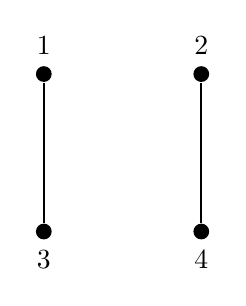
\begin{tikzpicture}[
       thick,
       acteur/.style={
         circle,
         fill=black,
         thick,
         inner sep=2pt,
         minimum size=0.2cm
       }
     ]

       \node (a1) at (0,0) [acteur,label=below:3]{};
       \node (a2) at (0,2)[acteur,label=above:1]{}; 
       \node (a3) at (2,2) [acteur,label=above:2]{}; 
       \node (a4) at (2,0) [acteur,label=below:4]{}; 
  
       \draw (a1) -- (a2); 
       \draw (a3) -- (a4); 

\end{tikzpicture}
  \caption{The support of a $1$-cosystole, which can not be determined using disjoint cycles}
  \label{figure6:Figure 6}
\end{figure}


Even though we can not determine all cosystoles by this "disjoint cycles" method, there is a conjecture, that we might be able to determine all Cheeger cosystoles this way, except for the cases when \(k=n-3\), since all the Cheeger cosystoles we know until now could be determined like that (see \cite{1} and \cite{6}).\\
Finding large families of cycles with pairwise disjoint supports is a problem, that has been for example approached by Peter Keevash (see \cite{11}), who determined the number of vertices \(n\), for which it is possible to partition the uniform \(k\)-skeleton of \(\Delta^{[n]}\), such that every part is the boundary of a (\(k+1\))-simplex.\\
For the case of cut-minimal graphs it might be easier to find large families of edge-disjoint cycles, but since we are not only interested in finding cut-minimal graphs but Cheeger graphs, we still have to handle the challenge of constructing graphs \(G\) by choosing edges in those cycles, such that the number \(T(G)\) becomes as small as possible.

\section{Find maximal cosystoles of a simplex}

In Theorem \ref{theorem1} we determined the maximum number of edges a cut-minimal graph can have and even discovered the unique (up to isomorphy) shape of such a graph. It always consists of two disjoint as equally large as possible complete graphs. For higher-dimensional cosystoles by now we have no idea about the largest possible norm and how those cosystoles look like.
\section{The case when n is a power of 2}

\section{The shape of Cheeger cosystoles}

\section{Cheeger constants for other complexes}

